\documentclass{article}
\usepackage[ngerman]{babel}
\usepackage[utf8]{inputenc}
\usepackage{graphicx} 
\usepackage{epstopdf}
\usepackage{svg}
\usepackage{svg}
\usepackage{booktabs}
\usepackage{longtable, lscape}
\usepackage{tikz}
\usepackage{multicol}
\usepackage{longtable}
\usepackage{array} 
\usepackage{tabularx}
\usepackage{varwidth}
\graphicspath{{img/}}
\usepackage{geometry}
\usepackage{amsmath,mathtools}
\usepackage{pdflscape}
\geometry{a4paper, top=25mm, left=30mm, right=25mm, bottom=20mm}


\begin{document}
\section{Komplementär-Filter}
\subsection{Vorwort}
In dem ersten Teil wird aus dem üblichen Blockschaltbild die bekannte Berechnungsvorschrift hergeleitet. Anschließend werden ein allgemein gültiges Blockschaltbild und Entwurfsregeln vorgestellt, welche an zwei Beispielen demonstriert werden.

\subsection{Herleitung Berechnungsvorschrift aus dem Blockschaltbild}
Bei der Erklärung des Komplementär-Filters wird in der Regel lediglich das folgende Blockschaltbild aufgezeigt (normalerweise fehlen die Übertragungsfunktionen). 

\begin{figure}[!h]
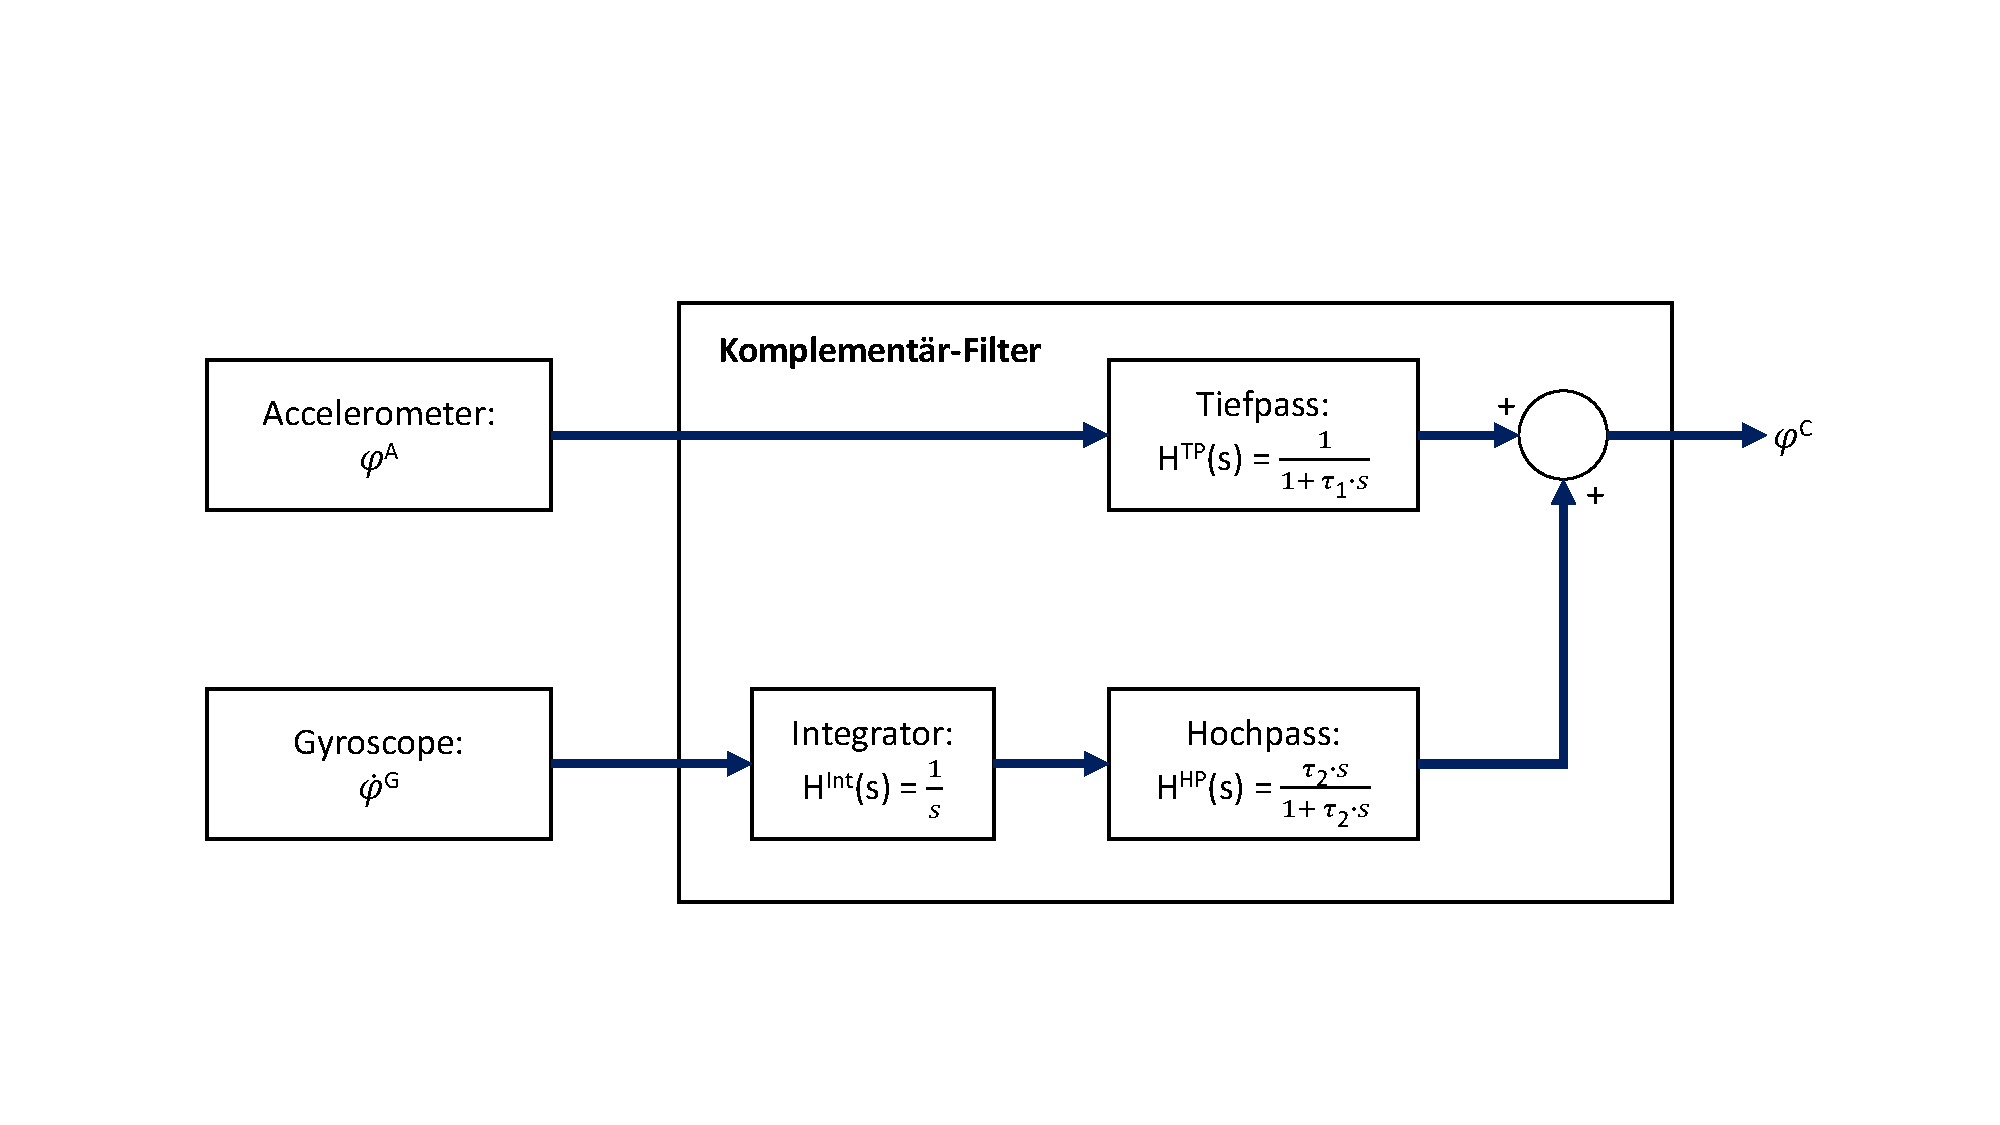
\includegraphics[scale=0.5,trim={0 3cm 0 4cm},clip]{Komp_CuBa_1D}

\end{figure}

Standard-Erklärung: 

Über die Beschleunigungssensoren wird der Winkel $\varphi^A$ geschätzt, welcher allerdings von hochfrequenten Rauschsignalen beeinflusst ist (vermutlich beginnt der Aufbau durch die oszillierenden Motormomente zu vibrieren, was nicht in dem mathematischen Modell erfasst wird). Deshalb wird dieser Winkel mit Hilfe eines Tiefpasses gefiltert. Andererseits kann der Winkel auch über die Integration der Winkelgeschwindigkeit $\dot{\varphi}^G$ ermittelt werden, diese Berechnung leidet allerdings unter einem konstanten Drift, welcher durch den Offset des Gyroscope entsteht. Durch eine Hochpassfilterung soll diese niederfrequente Störung eliminiert werden. 
In den üblichen Erläuterungen folgt auf diese Erklärung die Berechnungsvorschrift, welche allerdings nicht aus dem Blockschaltbild hergeleitet wird.

\begin{equation}
\label{Komp_BV_eq}
\varphi^C_n = \alpha \cdot (\varphi^C_{n-1} + T \cdot \dot{\varphi}^G) + (1-\alpha) \cdot \varphi^A
\end{equation}

Im folgenden wird deshalb eine Herleitung der Berechnungsvorschrift nach [WietzkeZettel] dargestellt.
\newline

Im Bildbereich ergibt sich aus dem Blockschaltbild der folgende Zusammenhang.

\begin{equation}
\varphi^C(s) = \frac{1}{1 + \tau_1 \cdot s} \cdot \varphi^A(s) + \frac{\tau_2 \cdot s}{1 + \tau_2 \cdot s} \cdot \frac{1}{s} \cdot \dot{\varphi}^G(s)
\end{equation}

Das Hochpass-Filter und der Integrator können zu einem Tiefpass zusammengeführt werden.

\begin{equation}
\label{Comp_Bild_eq}
\varphi^C(s) = \frac{1}{1 + \tau_1 \cdot s} \cdot \varphi^A(s) + \frac{\tau_2}{1 + \tau_2 \cdot s} \cdot \dot{\varphi}^G(s)
\end{equation}

Die Differentiation kann im zeitdiskreten Bereich wie folgt dargestellt werden.

\begin{equation}
\dot{y}(t) = \frac{y_n - y_{n-1}}{T} 
\end{equation}

Im Bildbereich entspricht dies der Backward-Euler-Transformation.

\begin{equation}
s = \frac{1 - z^{-1}}{T}
\end{equation}

Dadurch kann (\ref{Comp_Bild_eq}) als Z-Transformierte dargestellt werden.

\begin{equation}
\begin{split}
\varphi^C(z) & = \frac{1}{1 + \tau_1 \cdot \frac{1 - z^{-1}}{T} } \cdot \varphi^A(z) + \frac{\tau_2}{1 + \tau_2 \cdot \frac{1 - z^{-1}}{T}} = \\
& = \frac{T}{T + \tau_1 - \tau_1 \cdot z^{-1}} \cdot \varphi^A(z) + \frac{\tau_2 \cdot T}{T + \tau_2 - \tau_2 \cdot z^{-1}} \cdot \dot{\varphi}^G(z)
\end{split}
\end{equation}

Unter der Annahme das die Zeitkonstante des Tiefpass $\tau_1$ und des Hochpass $\tau_2$ identisch sind (hierher vermutlich der Name Komplementär-Filter) kann weiter vereinfacht werden.
\begin{equation}
\tau = \tau_1 = \tau_2
\end{equation}
\begin{equation}
\begin{split}
(T + \tau - \tau \cdot z^{-1}) \cdot \varphi^C(z) = T \cdot \varphi^A(z) + \tau \cdot T \cdot \dot{\varphi}^G(z)
\end{split}
\end{equation}
\begin{equation}
(T + \tau) \cdot \varphi^C(z) = \tau \cdot [\varphi^C(z) \cdot z^{-1}  + T \cdot \dot{\varphi}^G(z)] + T \cdot \varphi^A(z)
\end{equation}
\begin{equation}
\begin{split}
\varphi^C(z) & = \frac{\tau}{\tau + T}[\varphi^C(z) \cdot z^{-1}  + T \cdot \dot{\varphi}^G(z)] + \frac{T}{T + \tau} \varphi^A(z) \\
& = \frac{\tau}{\tau + T}[\varphi^C(z) \cdot z^{-1}  + T \cdot \dot{\varphi}^G(z)] + (1 - \frac{\tau}{T + \tau}) \varphi^A(z)
\end{split}
\end{equation}
Durch die Substitution $\alpha = \frac{\tau}{\tau + T}$ kann weiter vereinfacht werden. Welche in zeit diskreter Darstellung der Berechnungsvorschrift (\ref{Komp_BV_eq}) entspricht.

\begin{equation}
\varphi^C(z)  = \alpha[\varphi^C(z) \cdot z^{-1}  + T \cdot \dot{\varphi}^G(z)] + (1 - \alpha) \varphi^A(z)
\end{equation}
\begin{equation}
\varphi^C_n = \alpha(\varphi^C_{n-1}  + T \cdot \dot{\varphi}^G_n) + (1 - \alpha) \varphi^A_n
\end{equation}

\subsection{Vorschlag: Allgemeine Entwurfsregel für Komplementär-Filter}
Angenommen es wird ein Filter nach dem folgenden Blockschaltbild entworfen, wobei das Signal $w$ gesucht ist. Die beiden Eingangssignale $x^{C1}$ und $x^{C2}$ setzten sich jeweils aus $w$ und einem Rauschsignal $x^{R1}$ bzw. $x^{R2}$ zusammen.

\begin{figure}[!h]
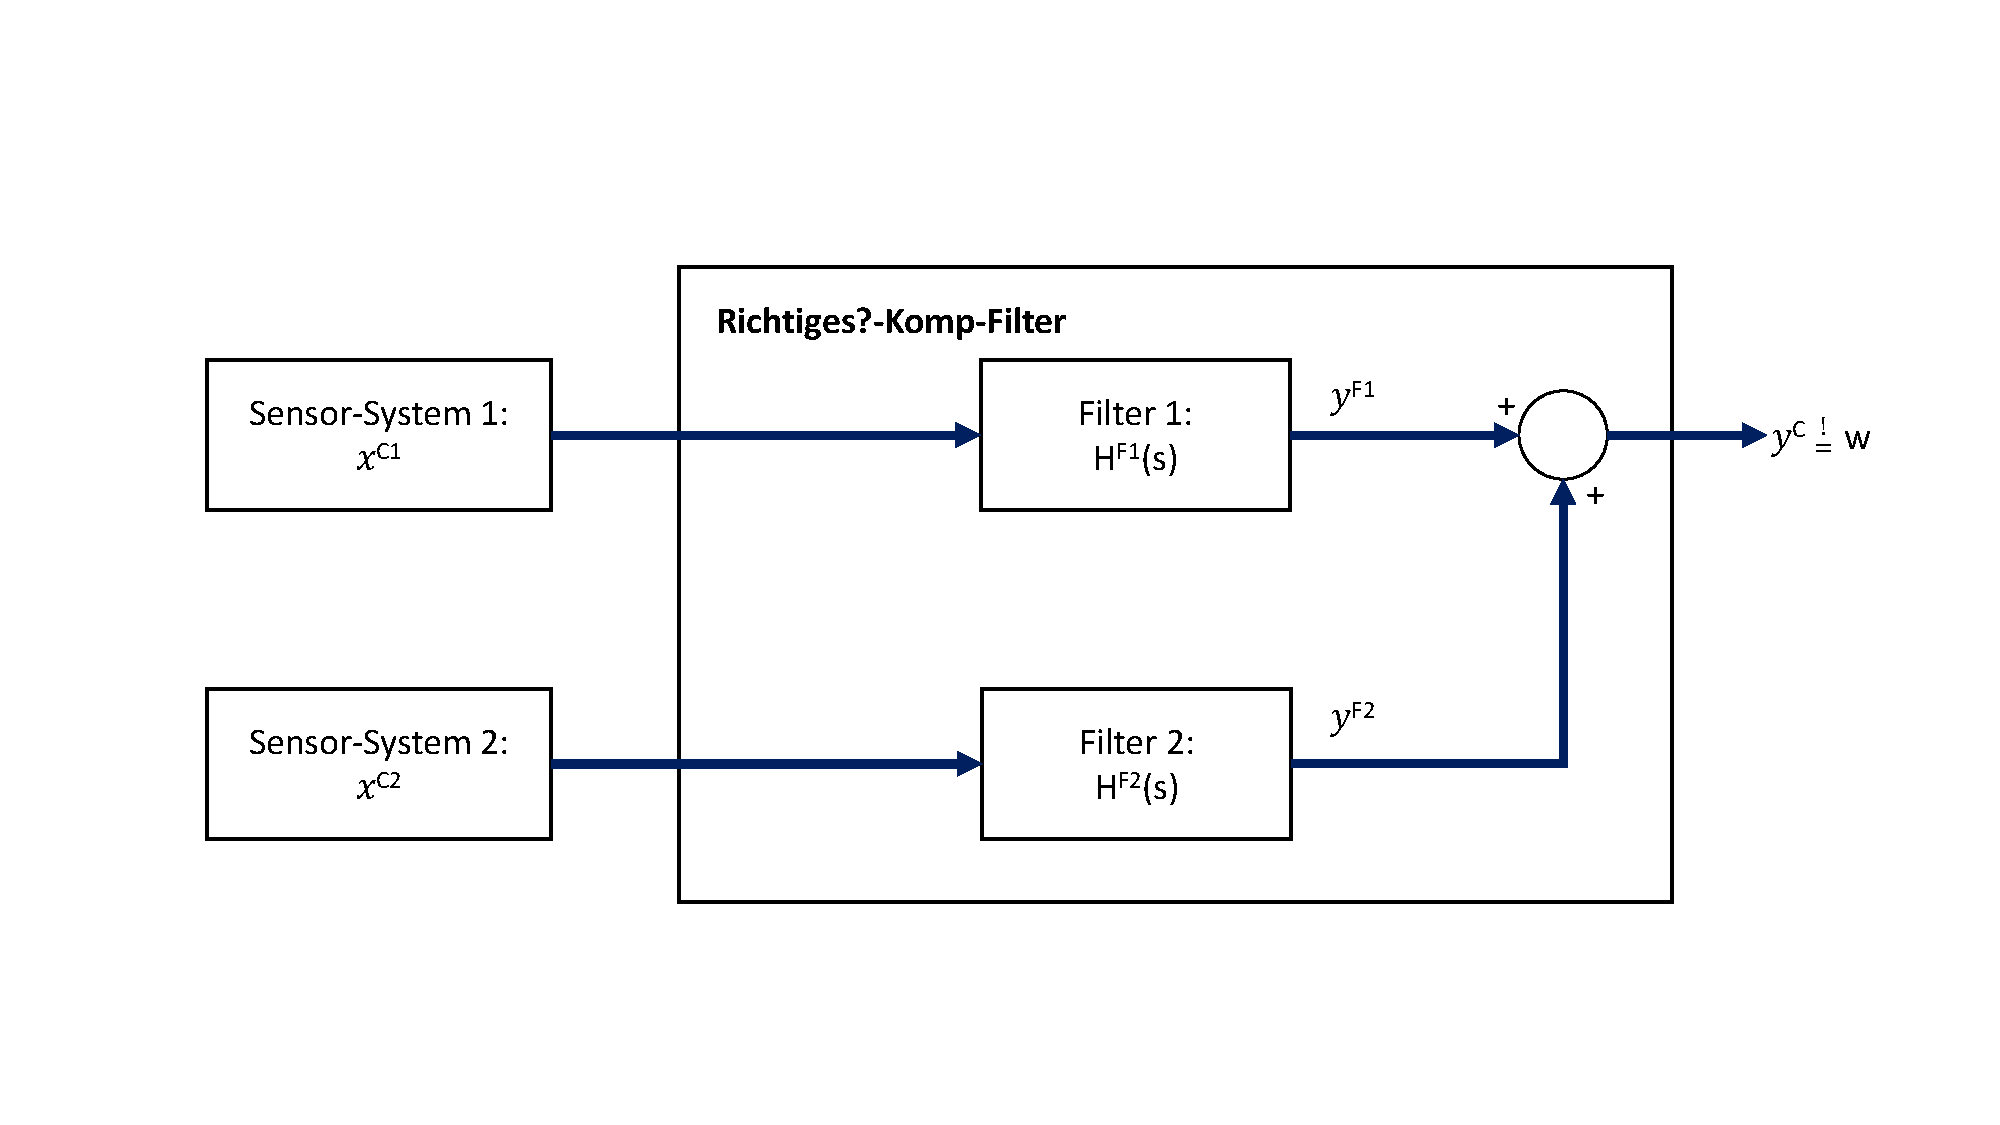
\includegraphics[scale=0.5,trim={0 3cm 0 4cm},clip]{Allg_Komp}
\end{figure}

\begin{equation}
x^{Ci} = w + x^{Ri} 
\end{equation}
Daraus folgt für die Ausgangssignale der Filter:
\begin{equation}
y^{Fi}(s) = H^{Fi} \cdot x^{Ci} = H^{Fi} \cdot (w + x^{Ri}) 
\end{equation}
Insofern es sich bei den Filter um lineare System handelt gilt das Distributivgesetz.
\begin{equation}
y^{Fi}(s) = H^{Fi} \cdot w + H^{Fi} \cdot x^{Ri} 
\end{equation}
Die erste Forderung an die Filter ist, dass die Rauschanteile eliminiert werden.
\begin{equation}
\label{comp_rule_1}
H^{Fi} \cdot x^{Ri} \overset{!}{=} 0
\end{equation}
Das Ausgangssignal $y^C$ des Gesamtsystem kann wie folgt berechnet werden.
\begin{equation}
y^C(s) = H^{F1}(s) \cdot x^{C1}(s) + H^{F1}(s) \cdot x^{C2}(s) = H^{F1}(s) \cdot [w(s) + x^{R1}(s)] + H^{F2}(s) \cdot [w(s) + x^{R2}(s)]
\end{equation}
Falls die Bedingung (\ref{comp_rule_1}) erfüllt ist fallen die Rauschterme weg.
\begin{equation}
y^C(s) = H^{F1}(s) \cdot w(s) + H^{F2}(s) \cdot w(s) = w \cdot [H^{F1}(s) + H^{F2}(s)]
\end{equation}
Wenn nun die zweite Forderung 
\begin{equation}
\label{comp_rule_2}
H^{F1}(s) + H^{F2}(s) \overset{!}{=} 1
\end{equation}
erfüllt ist, ist das Ausgangssignal $y^C$ gleich dem gesuchten Signal $w$ (wenn diese Bedingung erfüllt ist ergibt auch der Name Komplementär-Filter Sinn). Prinzipiell kann die Summe der Übertragungsfunktionen auch ein beliebiger, konstanter Wert $a \in \rm I\!R$ sein, dann gilt $y^C = a \cdot w$. Bleibt allerdings ein von $s$ abhängiger Term übrig (wäre der Fall bei dem Würfelbeispiel, falls $\tau_1 \neq \tau_2$) so würde gelten:
\begin{equation}
y^C(s) = H^C(s) \cdot w(s)
\end{equation}
Somit wäre der Zusammenhang von $y^C$ und $w$ von dem momentanen Frequenzspektrum von $w$ abhängig, welches sich praktisch kaum ohne Verzögerung bestimmen lässt.


\subsection{Beispiel: Filter um Winkel $\varphi$ des Würfels zu bestimmen}
Für den Würfel bestehen zwei Wegen den Winkel $\varphi$ zu bestimmen, einerseits die Schätzung aus den Beschleunigungswerten $\varphi^A$, andererseits die Integration der Winkelgeschwindigkeit $\dot{\varphi}^G$.

Im ersten Schritt müssen die Spektren der Rauschanteile bestimmt werden, dafür kann der Würfel auf die Seite gelegt werden ($\dot{\varphi} = 0$). Werden in dieser fixen Lage die Gyroscope-Werte aufgezeichnet und integriert kann das Spektrum des Rauschens berechnet werden. 
Bei der zweiten Messung liegt der Würfel ebenfalls auf der Seite, nun werden die Motoren mit einem Pulssignal angesteuert. Da das Gravitationsmoment in der Seitenlage zu groß ist, führt das Motormoment zu keiner Winkelbeschleunigung ($\ddot{\varphi}=0$). Werden die Accelerometer nun mit einer ausreichend großen Frequenz abgetastet kann das Rauschsignal ermittelt werden (theoretisch; müssen wir noch ausprobieren wie gut das funktioniert).

Diese Analyse sollte dann ergeben, dass das Gyroscope von niederfrequenten Rauschen $x^{R1}$ und die Accelerometer von hochfrequenten Rauschen $x^{R2}$ betroffen sind. Deshalb bietet sich die Kombination aus Hoch- und Tiefpass an.

\begin{equation}
\begin{split}
x^{C1}(s) = \varphi^A(s) + x^{R2}(s) \hspace{80pt} & x^{C2}(s) = \frac{1}{s} \dot{\varphi}^G(s) + x^{R1}(s)  \\
H^{F1}(s) = H^{TP}(s) = \frac{1}{1 + \tau_1 \cdot s} \hspace{80pt} & H^{F1}(s)=H^{RP}(s) = \frac{\tau_2 \cdot s}{1 + \tau_2 \cdot s}
\end{split}
\end{equation}

Die Werte $\tau_1$ und $\tau_2$ müssen nach (\ref{comp_rule_1}) so gewählt werden, dass die Rauschterme verschwinden. Außerdem muss nach (\ref{comp_rule_2}) folgende Beziehung gelten.

\begin{equation}
\begin{split}
1 & \overset{!}{=}  H^{TP}(s) + H^{HP}(s) = \frac{1}{1 + \tau_1 \cdot s} + \frac{\tau_2 \cdot s}{1 + \tau_2 \cdot s}
\end{split}
\end{equation}

Diese Bedingungen ist nur erfüllt wenn die Werte $\tau_1$ und $\tau_2$ identisch sind.

\newpage
\subsection{Beispiel: Filter um Winkelgeschwindigkeit $\dot{\varphi}$ zu bestimmen}
Die Winkelgeschwindigkeit des Würfels ergibt sich einerseits aus den Gyroscope-Werten, andererseits aus den integrierten Winkelbeschleunigungen welche aus den Accelerometer-Werten berechnet werden können. Es wird angenommen, dass die Rauschsignale und somit auch die Filter identisch zu dem vorherigen Beispiel sind.

\begin{figure}[!h]
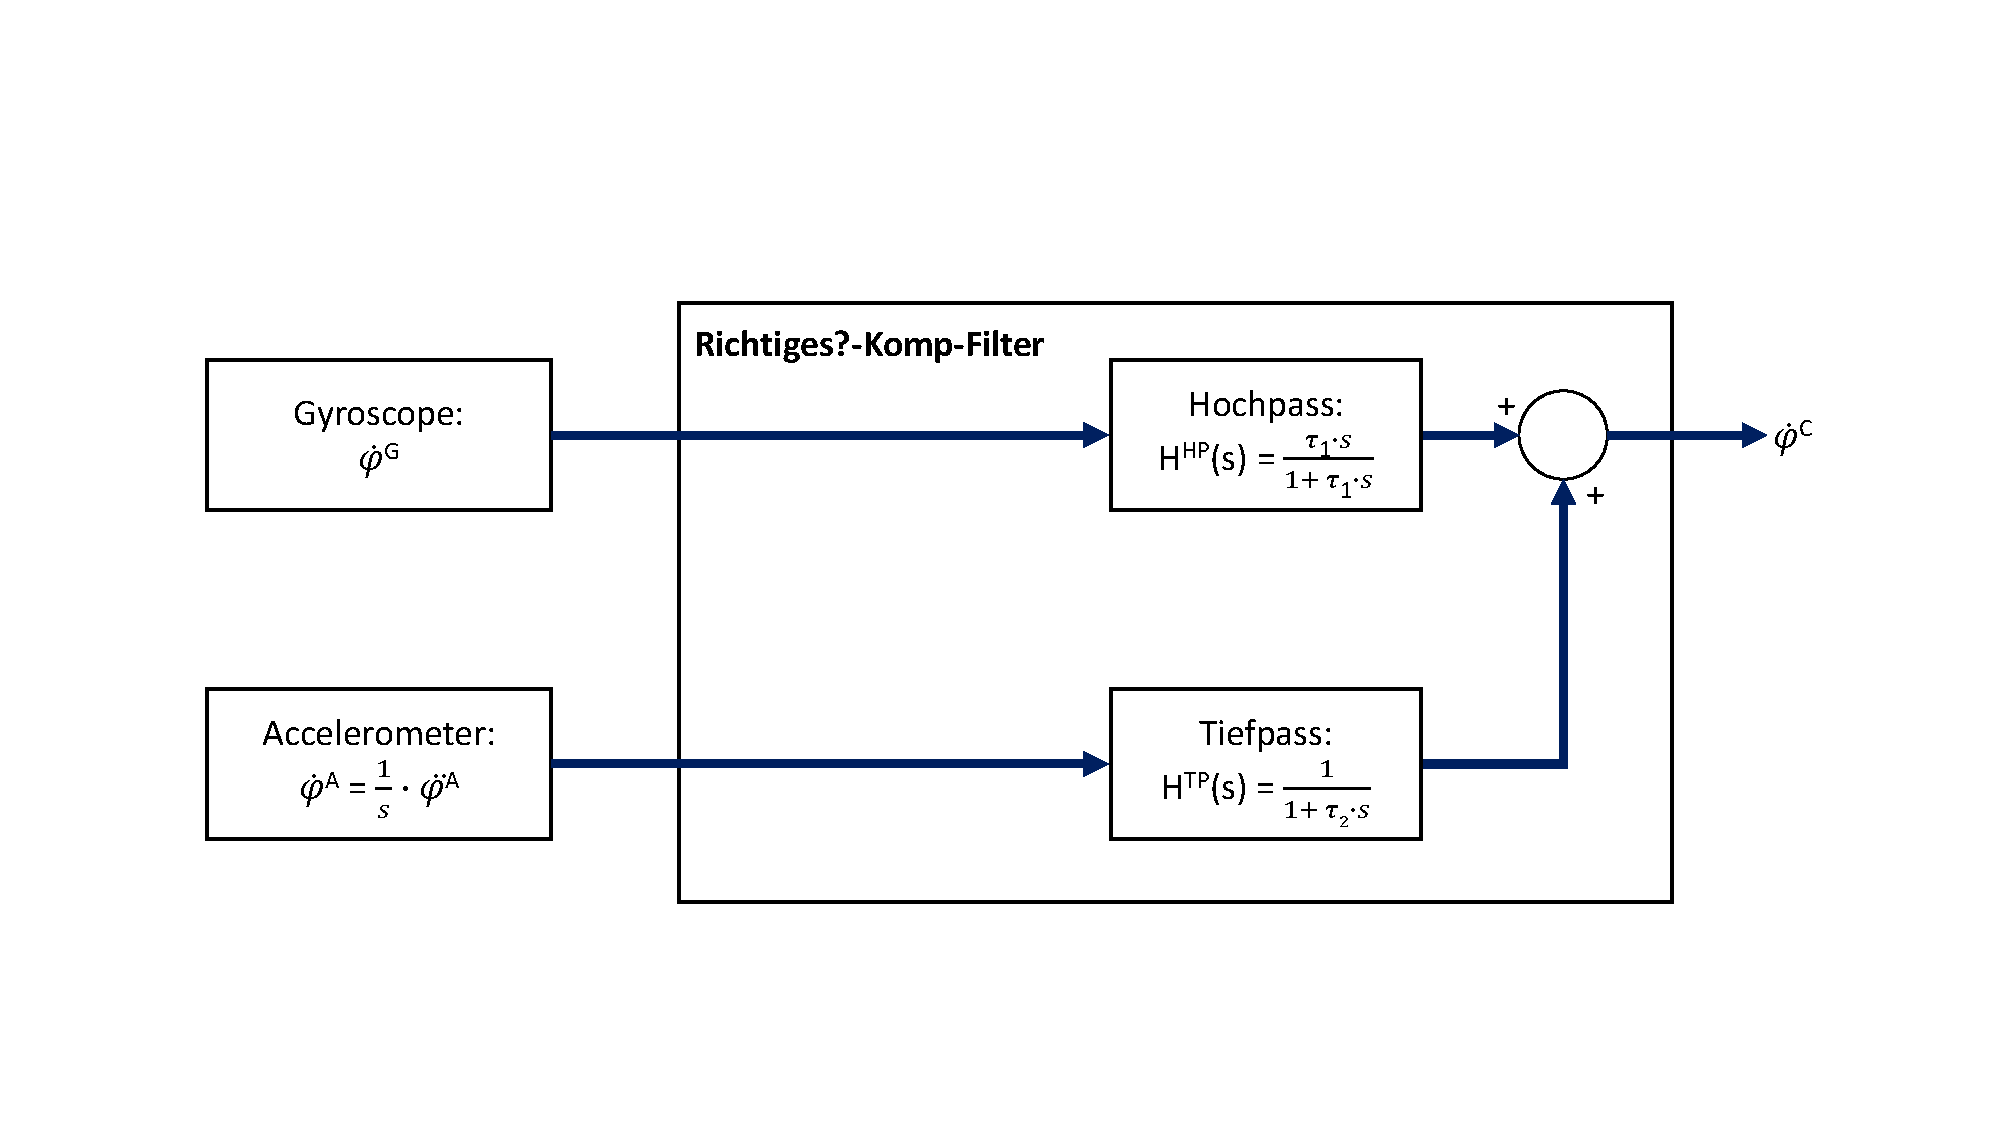
\includegraphics[scale=0.5,trim={0 3cm 0 4cm},clip]{Komp_CuBa_phi__d}
\end{figure}

Um (\ref{comp_rule_2}) zu erfüllen muss ebenfalls $\tau_1 = \tau_2 = \tau$ gelten. Somit ergibt sich folgender Zusammenhang zwischen den Sensorwerten und dem Ausgangssignal des Komplementär-Filters.
\begin{equation}
\begin{split}
y^C(s) &= \frac{\tau_1 \cdot s}{1 + \tau_1 \cdot s} \cdot \dot{\varphi}^G(s) + \frac{1}{1+\tau_2 \cdot s} \cdot \dot{\varphi}^A(s) \\
&= \frac{\tau \cdot s}{1 + \tau \cdot s} \cdot \dot{\varphi}^G(s) + \frac{1}{1+\tau \cdot s} \cdot \dot{\varphi}^A(s)
\end{split}
\end{equation}
\begin{equation}
\frac{T+\tau}{\tau} \cdot y^C(s) = \frac{\tau}{T} \cdot s \cdot \dot{\varphi}^G(s) + \dot{\varphi}^A(s)
\end{equation}
Mit Hilfe der Backward-Euler-Substitution (Tranformation?) $s = \frac{1-z^{-1}}{T}$ ergibt sich:
\begin{equation}
(1+\frac{\tau}{T}-\frac{\tau \cdot z^{-1}}{T}) \cdot \dot{\varphi}^C(z) = \frac{\tau}{T}\cdot (1-z^{-1}) \cdot \dot{\varphi}^G(z) + \dot{\varphi}^A(z)
\end{equation}
\begin{equation}
\frac{T+\tau}{T} \cdot \dot{\varphi}^C(z) = \frac{\tau}{T} \cdot z^{-1} \cdot \dot{\varphi}^C(z) + \frac{\tau}{T} \cdot (1-z^{-1}) \dot{\varphi}^G(z) + \frac{T}{T+\tau} \cdot \dot{\varphi}^A(z) 
\end{equation}
\begin{equation}
\dot{\varphi}^C(z) = \frac{\tau}{T+\tau} \cdot z^{-1} \cdot \dot{\varphi}^C(z) + \frac{\tau}{T + \tau} \cdot (1 - z^{-1}) \cdot \dot{\varphi}^G(z) + \frac{T}{T+\tau} \cdot \dot{\varphi}^A(z)
\end{equation}

\begin{equation}
\begin{split}
\dot{\varphi}^A_n &= \frac{T}{1-z^{-1}} \cdot \ddot{\varphi}^A_n \\
\dot{\varphi}^A_n - \dot{\varphi}^A_{n-1} &= T \cdot \ddot{\varphi}^A_n \\
\dot{\varphi}^A_n &= \dot{\varphi}^A_{n-1} + T \cdot \ddot{\varphi}^A_n
\end{split}
\end{equation}

\begin{equation}
\dot{\varphi}^C_n = \frac{\tau}{T+\tau} \cdot \dot{\varphi}^C_{n-1} + \frac{\tau}{T + \tau} \cdot (\dot{\varphi}^G_n + \dot{\varphi}^G_{n-1}) + (1 - \frac{\tau}{T + \tau}) \cdot (\dot{\varphi}^A_{n-1} + T \cdot \ddot{\varphi}^A_{n})
\end{equation}

Es kann auch wieder mit Hife von $\alpha = \frac{\tau}{T + \tau}$ substituiert werden, obwohl das doch sehr fragwürdig ist, da in der Allgemeinheit ja ganz gerne ein Standardwert für $\alpha$ verwendet wird . . . 

\begin{equation}
\dot{\varphi}^C_n = \alpha \cdot (\dot{\varphi}^C_{n-1} + \dot{\varphi}^G_n - \dot{\varphi}^G_{n-1}) + (1-\alpha) \cdot (\dot{\varphi}^A_{n-1} + T \cdot \ddot{\varphi}^A_n)
\end{equation}
\end{document}